\documentclass[tikz,border=6pt]{standalone}
\usepackage{tikz}
\usetikzlibrary{arrows.meta,positioning}
\definecolor{nebula}{HTML}{6366F1}
\definecolor{spark}{HTML}{14B8A6}
\definecolor{ink}{HTML}{334155}
\begin{document}
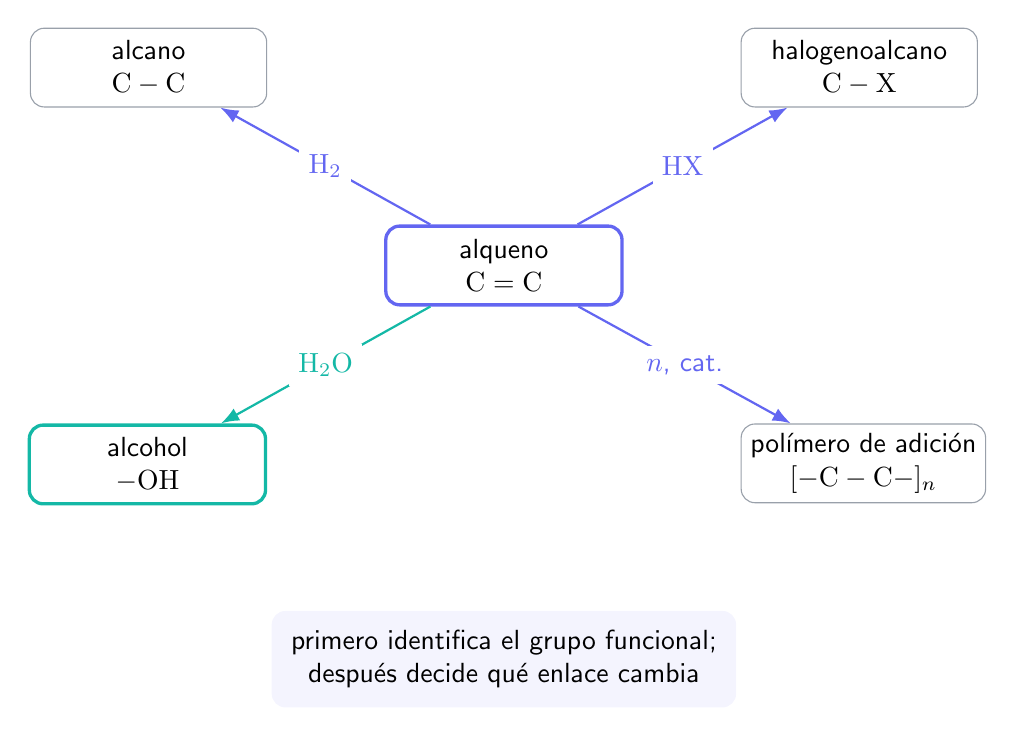
\begin{tikzpicture}[font=\sffamily,>=Latex,node distance=2.1cm,box/.style={draw=ink!50,rounded corners=5pt,minimum width=3cm,minimum height=1cm,align=center,fill=white}]
  \node[box,draw=nebula,very thick] (alkene) {alqueno\\$\mathrm{C=C}$};
  \node[box,above left=of alkene] (alkane) {alcano\\$\mathrm{C-C}$};
  \node[box,above right=of alkene] (halo) {halogenoalcano\\$\mathrm{C-X}$};
  \node[box,below left=of alkene,draw=spark,very thick] (alcohol) {alcohol\\$\mathrm{-OH}$};
  \node[box,below right=of alkene] (polymer) {pol\'imero de adici\'on\\$[-\mathrm{C-C}-]_n$};
  \draw[->,thick,nebula] (alkene)--(alkane) node[midway,fill=white] {$\mathrm{H_2}$};
  \draw[->,thick,nebula] (alkene)--(halo) node[midway,fill=white] {$\mathrm{HX}$};
  \draw[->,thick,spark] (alkene)--(alcohol) node[midway,fill=white] {$\mathrm{H_2O}$};
  \draw[->,thick,nebula] (alkene)--(polymer) node[midway,fill=white] {$n$, cat.};
  \node[align=center,fill=nebula!7,rounded corners=5pt,inner sep=7pt] at (0,-5) {primero identifica el grupo funcional;\\despu\'es decide qu\'e enlace cambia};
\end{tikzpicture}
\end{document}
